\documentclass[../../../../main.tex]{subfiles}
\begin{document}

\begin{flushright}
\footnotesize\textit{【自動文字起こし・要確認】}
\end{flushright}

\noindent
\textbf{[解]} $w = z^2 - 2z$ から $z = 1 \pm \sqrt{1+w}$ であるから,
\[
|z| \le \frac{5}{4} \iff |1 \pm \sqrt{1+w}| \le \frac{5}{4}
\]
だから, $\sqrt{1+w}$ の存在領域は右図斜線部 (境界含む). $\sqrt{1+w} = x + yi \; (x,y \in \mathbb{R})$ とおくと,
$w = (x^2 - y^2 - 1) + 2xy i$ で,
\[
|w|^2 = (x^2 - y^2 - 1)^2 + 4x^2 y^2
\]
これは $x \to -x, y \to -y$ について対称だから, $x \ge 0, y \ge 0$ で考えれば良い. この時,
\[
0 \le x \le \frac{1}{4}, \quad 0 \le y \le \sqrt{\left(\frac{5}{4}\right)^2 - (x+1)^2} \quad \cdots \textcircled{1}
\]
であり,
\[
|w|^2 = [ y^2 + (x+1)^2 ]^2 - 4x^2
\]
\textcircled{1}から $x$ を固定した時, $|w|^2$ は $y = \sqrt{\left(\frac{5}{4}\right)^2 - (x+1)^2}$ で最大で (軸が $y>0$ にある)
\begin{align*}
\max |w|^2 &= \left\{ 2x^2 + 2x - \frac{15}{16} \right\}^2 + 4x^2 \left\{ \frac{25}{16} - (x+1)^2 \right\} \\
&= -\frac{25}{4} x + \left(\frac{5}{4}\right)^2
\end{align*}
これは $x=0$ で $\max |w| = \frac{25}{16}$ をとる. したがって, $|w|$ が最大の時, $x=0, y=\frac{3}{4}$ でこの時
\[
w = -\frac{25}{16}
\]
である.

\begin{center}
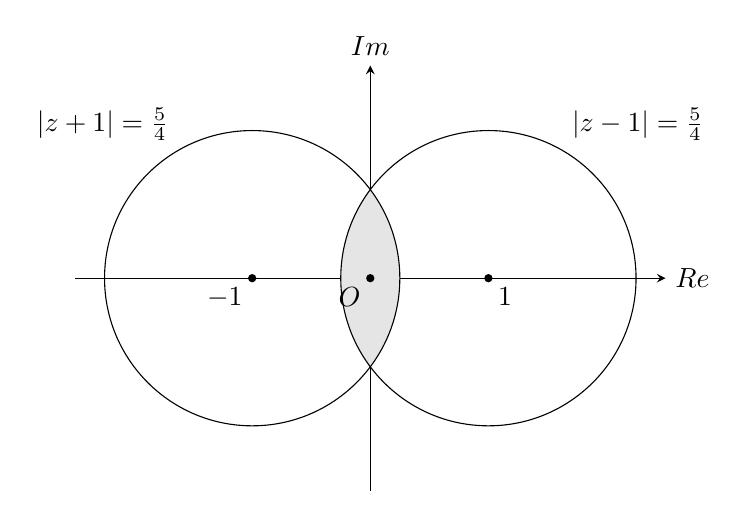
\begin{tikzpicture}[scale=1.5, >=stealth]
  \draw[->] (-2.5,0) -- (2.5,0) node[right] {$\text{Re}$};
  \draw[->] (0,-1.8) -- (0,1.8) node[above] {$\text{Im}$};
  \begin{scope}
    \clip (-1,0) circle (1.25);
    \fill[gray!20] (1,0) circle (1.25);
  \end{scope}
  \draw (-1,0) circle (1.25);
  \draw (1,0) circle (1.25);
  \node[above left] at ({-1 + 1.25*cos(120)}, {1.25*sin(120)}) {$|z+1|=\frac{5}{4}$};
  \node[above right] at ({1 + 1.25*cos(60)}, {1.25*sin(60)}) {$|z-1|=\frac{5}{4}$};
  \fill (-1,0) circle (1pt) node[below left] {$-1$};
  \fill (1,0) circle (1pt) node[below right] {$1$};
  \fill (0,0) circle (1pt) node[below left] {$O$};
\end{tikzpicture}
\end{center}

\bigskip

\noindent
\textbf{[解2]} $z$ の2次方程式 $z^2 - 2z - w = 0$ の2解を $z_1, z_2$ とする.
\[
\begin{cases}
z_1 + z_2 = 2 \\
z_1 z_2 = -w
\end{cases} \quad \cdots \textcircled{1}
\]
ならば $|z_1|, |z_2| \le \frac{5}{4}$ となるような $w$ をかんがえれば良い.
\[
|w| = |-z_1 z_2| = |z_1| |z_2| \le \frac{25}{16}
\]
等号成立する時, $z_1, z_2 = 1 \pm \frac{3}{4}i$ で十分. この時 $w = -\frac{25}{16}$. \hfill $\qed$

\end{document}
